% !TeX root = ../main.tex

\chapter{石墨烯和量子霍尔效应}


量子霍尔效应是物理学中非常重要的研究方向,而石墨烯与之紧密相关。例如,在$2005$年,Novoselov等\cite{RN18}和张远波等\cite{RN19}在石墨烯中观测到了量子霍尔效应,Kane和Mele研究了石墨烯的量子自旋霍尔效应\cite{RN20}。在这一章节中我们将简单介绍量子霍尔效应的研究与发展,且不仅仅局限于石墨烯这一种材料。

\section{经典霍尔效应}

在讨论量子霍尔效应之前,我们先介绍经典霍尔效应。

$1879$年,Hall发现Hall电阻与外加的垂直磁场成线性关系\cite{RN21}:
\begin{equation}
    R_H=\frac{B}{qnd}
\end{equation}
式中,$q$是载流子电荷量,$n$是载流子面密度。

\begin{figure}
    \centering
    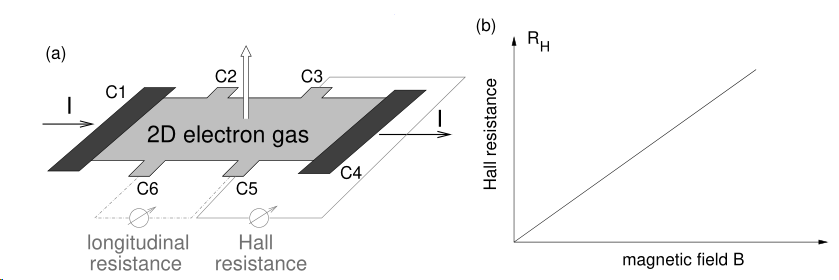
\includegraphics[scale=0.5]{img/Hall}
    \caption{经典霍尔效应}
\end{figure}

通过Drude模型我们可以对经典霍尔效应进行解释。

考虑载流子为电子,电子受到电场力和洛伦兹力,我们得到
\begin{equation}
    \dv{\vb p}{t}=-e\left(\vb E+\frac{\vb p}{m}\times\vb B\right)-\frac{\vb p}{\tau}
\end{equation}

我们希望求得稳定解,因此令$\dv{\vb p}{t}=0$。如果假设磁场在$z$方向上,我们会在$x\textendash y$方向上得到如下关系:
\begin{align*}
    eE_x & = -\frac{eB}{m}p_y-\frac{p_x}{\tau} \\
    eE_y & = -\frac{eB}{m}p_x-\frac{p_y}{\tau}
\end{align*}

我们把
\begin{equation}
    \omega_C=\frac{eB}{m}
\end{equation}
称为电子的回旋频率。

考虑到Drude模型中的电导率
\begin{equation}
    \sigma_0=\frac{ne^2\tau}{m}
\end{equation}
有
\begin{align*}
    \sigma_0 E_x & = -en\frac{p_x}{m}-en\frac{p_y}{m}(\omega_C\tau) \\
    \sigma_0 E_y & = en\frac{p_x}{m}(\omega_C\tau)-en\frac{p_y}{m}
\end{align*}

由于电流密度
\begin{equation}
    \vb j=-en\frac{\vb p}{m}
\end{equation}
代入上式就得到了电阻率
\begin{equation}
    \rho=\frac{1}{\sigma_0}\begin{pmatrix}
        1             & \omega_C\tau \\
        -\omega_C\tau & 1
    \end{pmatrix}
\end{equation}

因此Hall电阻率
\begin{equation}
    \rho_H=\frac{\omega_C\tau}{\sigma_0}=\frac{B}{en}
\end{equation}

\section{整数量子霍尔效应}

在经典霍尔效应发现之后,囿于技术原因,始终没有更进一步的结果。随着技术的进一步发展,特别是高质量的场效应晶体管的制造,在$1980$年,Klitzing等发现了整数量子霍尔效应\cite{RN30}。为此,Klitzing获得$1985$年诺贝尔物理学奖。

\subsection{研究过程与实验结果}

$1959$年,Atalla和Kahng在贝尔实验室发现了金属-氧化物半导体场效应晶体管(MOSFET),这使得人们可以研究近乎理想情况下的二维电子气中电子的情况。

$1975$年,Ando等对整数量子霍尔效应进行了预言\cite{RN30},但是他们当时对此表示怀疑。

$1980$年,Klitzing等在法国格勒诺布尔的强磁场实验室,利用MOSFET进行了实验。实验结果显示霍尔电导是严格量子化的,并且此性质非常稳定,与材料的几何尺寸等无关。\cite{RN22}

\subsection{理论解释}

对于整数量子霍尔效应,有若干不同的理论上的解释。$1981$年,Laughlin给出了一种解释\cite{RN23},后由Halperin进行完善\cite{RN24}。另一种是Thouless等提出的TKNN原理,我们将在后面进行叙述。

\section{量子自旋霍尔效应}

在整数量子霍尔效应中,一般要求较强的磁场,这限制了量子霍尔效应的实际应用。因此,人们开始考虑利用电子的
自旋自由度,在无外加磁场的情况下实现量子霍尔效应,此即量子自旋霍尔效应。与量子自旋霍尔效应紧密相关的是一类称为拓扑绝缘体的材料。在这一节中,我们将对这两者进行简单的叙述。

\subsection{拓扑绝缘体简述}

对固体按导电性进行分类,通常分为导体、半导体和绝缘体。然而,有一类相当特殊的材料,其内部是绝缘的,而边缘(对二维材料)或表面(对三维材料)是导电的,且这种特性相当稳定。上面这种材料就被称为拓扑绝缘体。对于拓扑绝缘体,研究其拓扑不变量是一件非常重要的事情。接下来两个小节中,我们将介绍拓扑绝缘体的拓扑不变量。

\subsection{TKNN原理}

$1982$年,Thouless、Kohmoto、Nightingale、Nijs提出了TKNN(以四人的姓氏首字母命名)原理\cite{RN25}。这一理论的提出,本意是解释Klitzing在$1980$年发现的整数量子霍尔效应。不过,这实际上也给出了拓扑绝缘体的一个不变量。虽然Thouless等当时并未提到拓扑的概念,但是在拓扑相变理论的逐渐完善下,人们意识到Thouless等给出了一个拓扑不变量——Chern数。这一结果也表明,拓扑绝缘体和量子霍尔效应有着非常紧密的联系。

我们可以从Berry相位\cite{RN26}和Bloch波函数$|u_m(\mathbf k)\rangle$开始考虑这个问题。Berry相位可以写成$\mathcal{A}_m=i\langle u_m|\nabla_k|u_m\rangle$的线积分,也可改写为Berry通量$\mathcal{F}_m=\nabla\times\mathcal{A}_m$的面积分。Chern数可以通过把Berry通量在布里渊区上积分得到:
\begin{equation}
    n_m=\frac{1}{2\pi}\int \dd[2]{\mathbf{k}\mathcal{F}_m}
\end{equation}
这是一个整数。

总Chern数即为各能带上Chern数之和:
\begin{equation}
    n=\sum_{m=1}^N n_m
\end{equation}

通过Kubo公式,可以证明霍尔电导
\begin{equation}
    \sigma_{xy}=ne^2/h
\end{equation}
因此它是量子化的。这说明了整数量子霍尔效应及其稳定性,给予Klitzing的实验结果一个很好的解释。

Hasan和Kane在\cite{RN27}中把这一结果与数学中的Gauss-Bonnet定理相对比。这两者运用的方法大致相同,得到的结果非常相似。同时,正是拓扑相关概念的引入使得这方面的问题有了明显进展。因此,TKNN原理可以被认为是数学和物理相结合的一个典型的例子。

\subsection{$Z_2$拓扑不变量}

如果Chern数非零,时间反演对称性将被打破。因此,找到时间反演对称下的拓扑不变量是很有必要的。$2005$年,Kane和Mele提出了$Z_2$拓扑不变量\cite{RN28}。

$Z_2$拓扑不变量的定义有若干种,我们在这里介绍一种\cite{RN29}。

为简单起见我们只考虑二维情形。定义酉矩阵
\begin{equation}
    w(\mathbf{k})=\langle u_m(\mathbf{k})|\Theta|u_n(-\mathbf{k})\rangle
\end{equation}

由布里渊区的几何性质,存在$4$个特殊点$\Lambda_a$,在这$4$个点处$\mathbf{k}$与$-\mathbf{k}$重合。由此可以推出$w(\Lambda_a)$是反对称的。

根据数学上的结果,如果我们定义
\begin{equation}
    \delta_a=\mathrm{Pf}(w(\Lambda_a))/\sqrt{\det(w(\Lambda_a))}
\end{equation}
那么$\delta_a$只能取$\pm1$。

于是,$Z_2$不变量定义为
\begin{equation}
    (-1)^v=\prod_{a=1}^{4}\delta_a
\end{equation}

\subsection{HgTe/CdTe}

量子自旋霍尔效应与拓扑绝缘体究竟有何联系?这个问题在\cite{RN28}和\cite{RN34}得到解答。作者预言,通过拓扑绝缘体可以实现量子自旋霍尔效应。并且,在\cite{RN34}中,作者指出,通过HgTe/CdTe超晶格结构可以实现量子自旋霍尔效应。

这在\cite{RN34}发表一年后得到了验证。$2007$年,德国Molenkamp研究组通过分子束外延生长法制备了CdTe/HgTe/CdTe超晶格,发现HgTe层具有临界宽度$d_c$:当$d<d_c$时,由于CdTe是半导体,样品几乎处于绝缘态;当$d>d_c$时,样品产生电导$2e^2/h$\cite{RN35}。具体图像可见图~\ref{fig:hgte}:

\begin{figure}
    \centering
    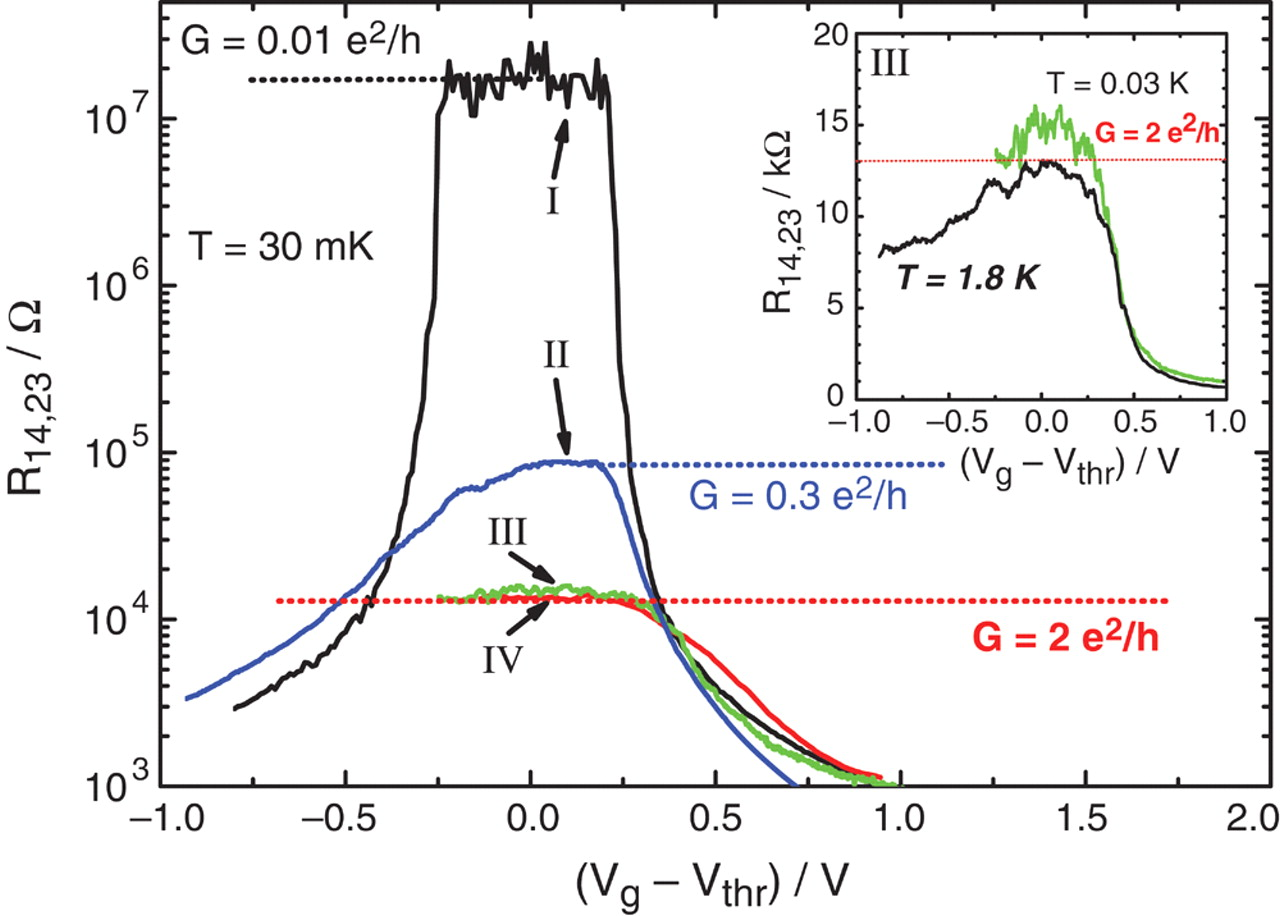
\includegraphics[scale=0.4]{img/HgTe+CdTe}
    \caption{HgTe/CdTe实验数据图像}
    \label{fig:hgte}
\end{figure}

此实验验证了HgTe/CdTe是二维拓扑绝缘体,被称为第一代拓扑绝缘体。

\subsection{三维拓扑绝缘体}

在HgTe/CdTe之后,人们开始研究三维拓扑绝缘体。由于这方面已不属于低维材料的范畴,我们只作简单介绍。

$2007$年,傅亮等预言铋锑合金是三维拓扑绝缘体\cite{RN36},于$2008$年被验证\cite{RN37}。$2009$年,中国科学院物理研究所的几位研究员预言$\mathrm{Bi}_2\mathrm{Se}_3$、$\mathrm{Bi}_2\mathrm{Te}_3$和$\mathrm{Sb}_2\mathrm{Te}_3$是拓扑绝缘体\cite{RN38}。同年,$\mathrm{Bi}_2\mathrm{Se}_3$被验证为拓扑绝缘体\cite{RN39},称为第二代拓扑绝缘体。$\mathrm{Bi}_2\mathrm{Te}_3$也同样得到验证\cite{RN40}。